\documentclass{article}
\usepackage{graphicx}
\usepackage{hyperref}
\usepackage{url}
\usepackage{listings}
\usepackage{subcaption}


\begin{document}

% First Page
\begin{titlepage}
\begin{figure}[!htb]
    \centering
    
\includegraphics[keepaspectratio=true,scale=0.75]{UCA_logo.png}
\end{figure}

\vspace{2mm}

\begin{center}
    {\LARGE \textbf{UNIVERSITÉ CÔTE D’AZUR}} \\[1mm]
    {\large DS4H} \\[1mm]
    {\LARGE \textbf{Master 1 Informatique}}
\end{center}

\vspace{10mm}

\begin{center}
    {\LARGE \textbf{Evaluating the Efficiency of Data Parallelism in Machine Learning within NEF}}
\end{center}

\vspace{10mm}

\begin{minipage}[t]{0.45\textwidth}
    {\large \textbf{Professor:}} \\[1mm]
    {Chuan XU} \\[2mm]
    {\large \textbf{Course:}} \\[1mm]
    {Distributed Memory Parallel Programming and its Applications}
\end{minipage}
\hfill
\begin{minipage}[t]{0.45\textwidth} \raggedleft
    {\large \textbf{Student Name:}} \\[1mm]
    {Yassin Es Saim} \\[2mm]
    {\large \textbf{Student ID:}} \\[1mm]
    {22109654}
\end{minipage}

\vspace{10mm}

\hrulefill

\vspace{2mm}

\begin{center}
    {\large \textbf{Year:}} \\
    {2024/2025}
\end{center}

\end{titlepage}
\thispagestyle{empty}
\newpage

\section{Introduction}
\subsection{Introduction to the NEF cluster}
The NEF cluster is a high-performance computing (HPC) environment provided by INRIA (Institut National de Recherche en Informatique et en Automatique). It is designed to support large-scale computational tasks, such as machine learning, data analysis, and scientific simulations. The cluster is equipped with both CPU and GPU nodes, which are optimized for different types of workloads. The CPU nodes feature multi-core processors, while the GPU nodes are equipped with high-performance GPUs, making the cluster suitable for parallel computing tasks.

The NEF cluster is built on a cluster computing approach, combining several generations of high-performance servers to create a heterogeneous parallel architecture. This architecture is enhanced by a fast network interconnect, high-capacity storage systems, and integration with Inria Sophia's interactive visualization platform. These features make NEF a powerful environment for tasks such as parallel computations, GPU-accelerated workloads, and sequential jobs.

NEF is part of the UCA OPAL distributed computation mesocentre, a collaborative initiative that expands its computational reach. The platform provides a robust software environment, supporting popular machine learning frameworks such as PyTorch and TensorFlow, as well as other scientific computing tools. Users can access the cluster's resources by submitting jobs through the OAR job scheduling system, which allows them to book nodes for their computations. This makes the NEF cluster an ideal platform for researchers and students to conduct experiments that require significant computational power.

For this project, the NEF cluster is particularly relevant because it provides the necessary hardware and software environment to evaluate the efficiency of data parallelism in machine learning. The ability to distribute workloads across multiple nodes and leverage parallel computing techniques makes the cluster a perfect testbed for measuring the impact of the number of computing devices and batch sizes on training time and throughput.

\subsection{Introduction to the nodes tested}
For this project, two types of nodes within the NEF cluster were tested: a \textbf{CPU node} and a \textbf{GPU node}. The CPU node \texttt{nef042.inria.fr} is part of the \textbf{Dell C6420 cluster}, which features dual-Xeon Skylake processors. The GPU node \texttt{nefgpu45.inria.fr} is part of the \textbf{Dell R740 GPU nodes}, which are equipped with high-performance GPUs and dual-Xeon Skylake or CascadeLake processors. These nodes were selected using the \textbf{Monika web interface}, which provides real-time information about resource availability in the NEF cluster.

To conduct the experiments, \textbf{8 CPU cores} were booked on the CPU node and \textbf{3 GPUs} were booked on the GPU node, as required by the task (explained in the next subsection). The nodes were reserved using the \textbf{OAR job scheduling system}, which allows users to allocate computational resources for a specified duration. Further details about the hardware specifications and configurations of these nodes will be provided in the \textbf{Evaluation} section.

\subsection{Introduction to the task}
The primary objective of this project is to evaluate the efficiency of data parallelism in machine learning, specifically within the NEF cluster. The task involves using the \textbf{DenseNet121 model} as a benchmark to measure the time taken for training with different configurations of computing devices and batch sizes. The experiments focus on understanding the impact of the number of computing devices and batch sizes on training time and throughput, rather than on training the model itself.

The \textbf{DenseNet121 model}, detailed later in the Evaluation section, is a convolutional neural network (CNN) known for its dense connections between layers, which allow for efficient feature reuse and parameter efficiency. The \textbf{Imagenette dataset}, a smaller subset of the ImageNet dataset, consists of 10 classes of images and is commonly used for benchmarking machine learning models. By using DenseNet121 and Imagenette, the experiments aim to evaluate how data parallelism can improve the efficiency of training deep learning models on distributed systems.

The following configurations were tested to evaluate data parallelism:
\begin{itemize}
    \item Varying the number of computing devices:
        \begin{itemize}
            \item CPU node: 1 to 8 cores
            \item GPU node: 1 to 3 GPUs
        \end{itemize}
    \item Testing different batch sizes on the GPU node: 16, 32, 64, and 128
\end{itemize}
The training time, computation+communication time, and throughput were measured for each configuration to analyze the efficiency of data parallelism. The results aim to identify the optimal configuration for efficient training and provide insights into the trade-offs between computational resources and training performance.

The following configurations were tested to evaluate data parallelism:
\begin{itemize}
    \item Varying the number of computing devices:
        \begin{itemize}
            \item CPU node: 1 to 8 cores
            \item GPU node: 1 to 3 GPUs
        \end{itemize}
    \item Testing different batch sizes on the GPU node: 16, 32, 64, and 128
\end{itemize}
The training time, computation+communication time, and throughput were measured for each configuration to analyze the efficiency of data parallelism. The results aim to identify the optimal configuration for efficient training and provide insights into the trade-offs between computational resources and training performance.

\section{Evaluation}
\subsection{Details of the node tested}
The experiments were conducted on two types of nodes within the NEF cluster, each with distinct hardware configurations:

\subsubsection{CPU Node}
\begin{itemize}
    \item \textbf{Node name}: \texttt{nef042.inria.fr}
    \item \textbf{Cluster}: Dell C6420 (2017)
    \item \textbf{Processor}: Dual-Xeon Skylake SP Silver 4114 @ 2.20GHz (20 cores per node)
    \item \textbf{Memory}: 64 GB RAM
    \item \textbf{Resources booked}: 8 CPU cores
\end{itemize}

\subsubsection{GPU Node}
\begin{itemize}
    \item \textbf{Node name}: \texttt{nefgpu45.inria.fr}
    \item \textbf{Cluster}: Dell R740 GPU nodes (2019)
    \item \textbf{Processor}: Dual-Xeon Silver 4110
    \item \textbf{Memory}: 96 GB RAM
    \item \textbf{GPUs}: 3x NVIDIA Tesla T4
    \item \textbf{Resources booked}: 3 GPUs
\end{itemize}

Both nodes are part of the NEF cluster's high-performance computing infrastructure, which includes a fast network interconnect (InfiniBand) and high-capacity storage systems to support large-scale machine learning tasks.

\subsection{Details of the training model tested}
The experiments utilized the \textbf{DenseNet121 model}, a variant of the DenseNet architecture with 121 layers. DenseNet (Dense Convolutional Network) is a deep neural network architecture known for its dense connections between layers, which allow for efficient feature reuse and parameter efficiency.

\subsubsection{Model architecture}
\begin{itemize}
    \item \textbf{Dense blocks}: the network consists of multiple dense blocks, where each layer is connected to every other layer in a feedforward manner. This ensures maximum information flow between layers.
    \item \textbf{Bottleneck layers}: each dense block contains bottleneck layers, which reduce the number of input feature maps and improve computational efficiency.
    \item \textbf{Transition layers}: between dense blocks, transition layers are used to reduce the number of feature maps and control the computational cost of the network.
    \begin{figure}[h!]
        \centering
            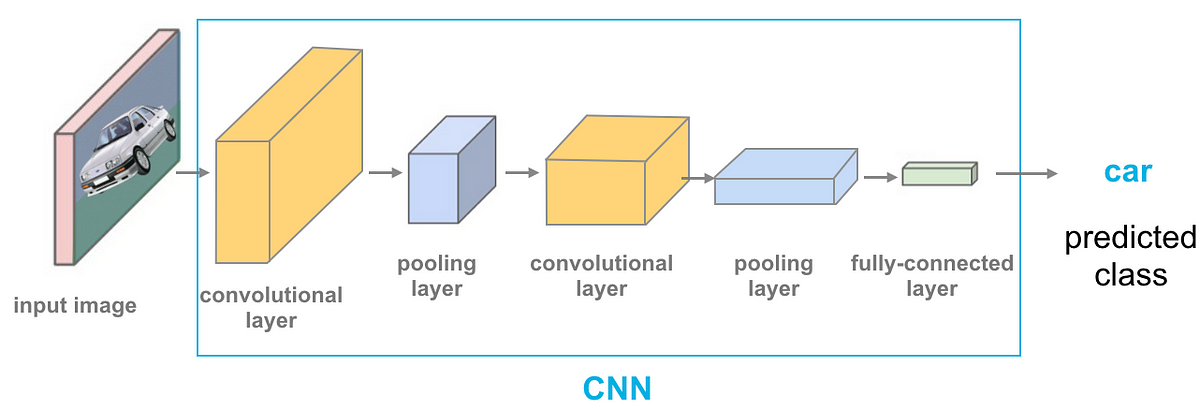
\includegraphics[width=\textwidth]{DenseNet121.png}
            \caption{a very general overview of a CNN illustrating the concept of convolutional layers, pooling layers, and fully-connected layers, which provides a foundation to understand the more complex architecture of DenseNet121.}
            \label{fig:cpu_time}
    \end{figure}
\end{itemize}



\subsubsection{Key features}
\begin{itemize}
    \item \textbf{Parameter efficiency}: DenseNet121 is designed to use fewer parameters compared to other deep networks, making it computationally efficient.
    \item \textbf{State-of-the-Art performance}: the DenseNet architecture has achieved state-of-the-art performance on various image classification tasks, including the ImageNet dataset.
    \item \textbf{PyTorch implementation}: the model was implemented using the \\ 
    \texttt{torchvision.models} module in PyTorch, which provides a pre-trained version of DenseNet121.
\end{itemize}

\section{Impact of the number of computing devices}

\subsection{Impact of the Computing Nodes}
The following four plots analyze the impact of the number of computing devices on training efficiency. The experiments were conducted with a fixed batch size of 32. For each task, 10 tests were performed, and the average values were taken to ensure reliable results.


\subsubsection{CPU plots}

% Two CPU plots side by side
\begin{figure}[h!]
    \centering
    \begin{subfigure}[b]{0.48\textwidth}
        \centering
        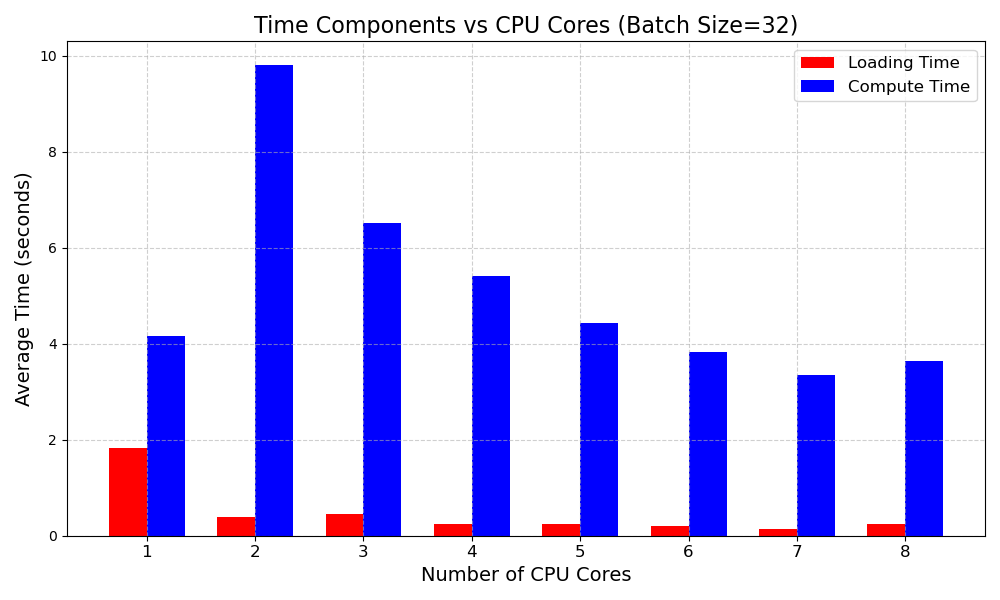
\includegraphics[width=\textwidth]{CPU/time_components_bar.png}
        \caption{Time (loading time, compute+communication time) vs number of CPU cores.}
        \label{fig:cpu_time}
    \end{subfigure}
    \hfill
    \begin{subfigure}[b]{0.48\textwidth}
        \centering
        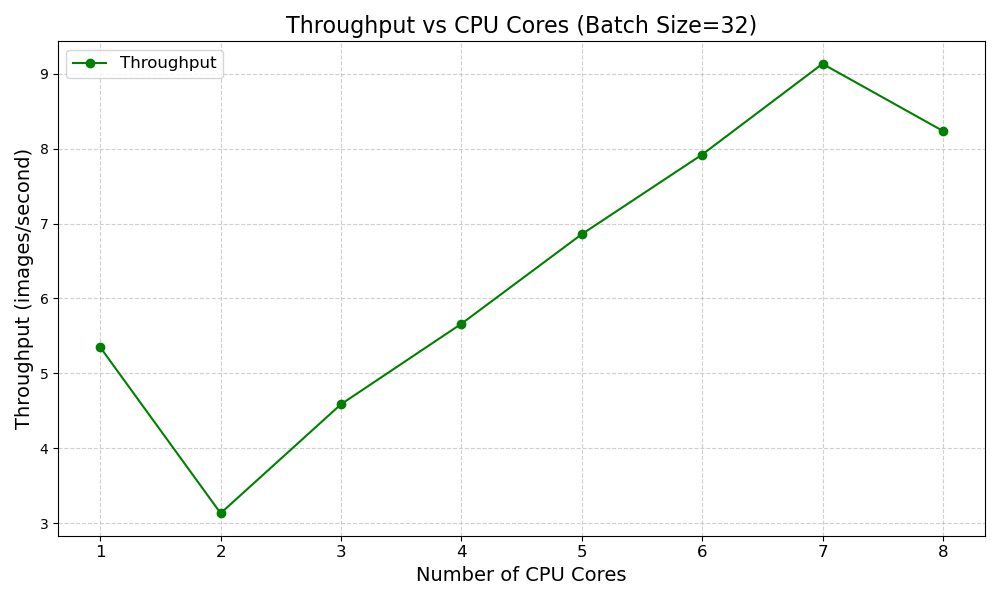
\includegraphics[width=\textwidth]{CPU/throughput_line.png}
        \caption{Throughput (batch size / time) vs number of CPU cores.}
        \label{fig:cpu_throughput}
    \end{subfigure}
    \caption{CPU performance metrics as a function of the number of cores.}
    \label{fig:cpu_plots}
\end{figure}

\subsubsection{GPU plots}

% Two GPU plots side by side
\begin{figure}[h!]
    \centering
    \begin{subfigure}[b]{0.48\textwidth}
        \centering
        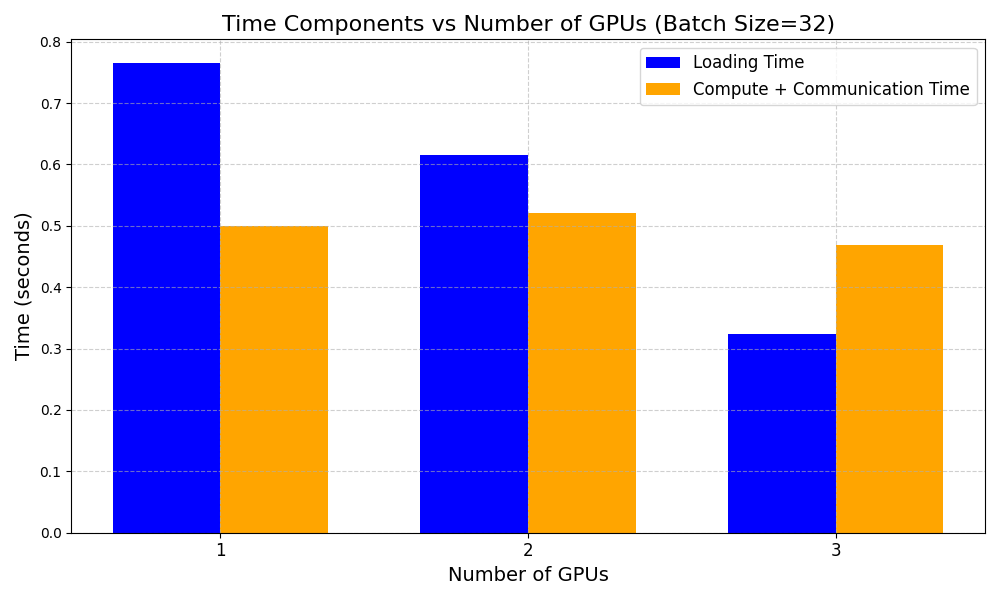
\includegraphics[width=\textwidth]{GPU/gpu_time_components_bar.png}
        \caption{Time (loading time, compute+communication time) vs number of GPU devices.}
        \label{fig:gpu_time}
    \end{subfigure}
    \hfill
    \begin{subfigure}[b]{0.48\textwidth}
        \centering
        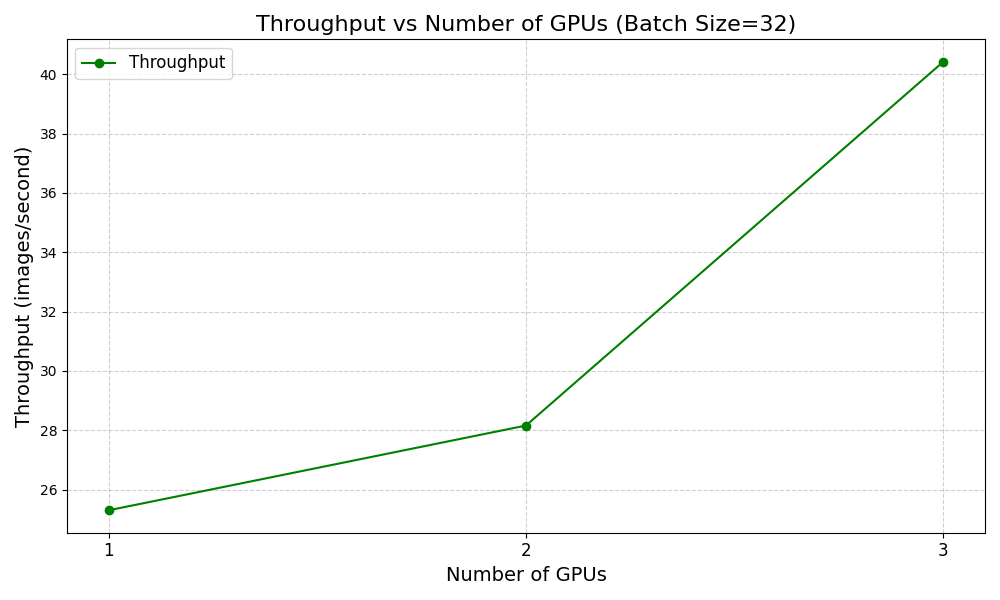
\includegraphics[width=\textwidth]{GPU/gpu_throughput_line.png}
        \caption{Throughput (batch size / time) vs number of GPU devices.}
        \label{fig:gpu_throughput}
    \end{subfigure}
    \caption{GPU performance metrics as a function of the number of devices.}
    \label{fig:gpu_plots}
\end{figure}



\subsubsection{CPU analysis}
\begin{itemize}
    \item \textbf{Time vs number of cores}:\\ as shown in Figure \ref{fig:cpu_time}, the compute+communication time decreases as the number of CPU cores increases, except for 8 cores, where it is slightly higher than for 7 cores. This anomaly can be attributed to several reasons, but the most probable one, based on research, is \textbf{resource contention} and \textbf{overhead in managing additional cores}. When all 8 cores are used, the system may experience increased contention for shared resources (e.g., memory bandwidth, cache), leading to higher communication overhead and slightly longer compute times. Additionally, the operating system's scheduling overhead may become more significant with 8 cores, further impacting performance.
    
    However, the loading time remains relatively constant when using more than 2 cores. This indicates that data parallelism effectively reduces computation time but has little impact on data loading, as loading is primarily I/O-bound and not significantly affected by the number of CPU cores.

    \item \textbf{Throughput vs number of cores}:\\ Figure \ref{fig:cpu_throughput} shows that the throughput increases linearly with the number of CPU cores, but it is slightly lower for 8 cores compared to 7 cores. This is consistent with the increase in compute+communication time observed for 8 cores. The slight drop in throughput can be explained by the \textbf{diminishing returns} of adding more cores. As the number of cores increases, the overhead of managing parallelism (e.g., thread synchronization, memory access contention) begins to outweigh the benefits of additional cores, leading to a small decrease in throughput.
\end{itemize}

\subsubsection{GPU analysis}
\begin{itemize}
    \item \textbf{Time vs number of devices}:
    as shown in Figure \ref{fig:gpu_time}, the loading time decreases significantly as the number of GPUs increases. This is likely due to the parallelization of data loading, where multiple GPUs can simultaneously load and process data, reducing the overall loading time. However, the compute+communication time decreases only slightly with more GPUs. This can be attributed to the communication overhead between GPUs, which becomes more significant as the number of devices increases. While parallel processing reduces computation time, the overhead of synchronizing data and gradients across multiple GPUs limits the overall improvement in compute+communication time.

    \item \textbf{Throughput vs number of devices}:
    Figure \ref{fig:gpu_throughput} shows that the throughput increases significantly with the number of GPUs.
    While the scaling is not perfectly linear, the results highlight the benefits of data parallelism for GPU-based training. For example, moving from 1 to 2 GPUs increases throughput by 40\%, and moving from 2 to 3 GPUs increases throughput by 50\%. These gains show that distributing the workload across multiple GPUs can significantly enhance performance, even if the scaling is not perfectly linear. This is a common characteristic of distributed systems, where the overhead of managing multiple devices is outweighed by the overall performance improvement.
\end{itemize}

\section{Impact of the Batch Size}

\subsection{Throughput vs number of GPUs for different Batch Sizes}
The following three plots analyze the impact of batch size on throughput for different numbers of GPUs. The experiments were conducted with batch sizes of 16, 64, and 128 on the GPU node. For each batch size and GPU configuration, 10 tests were performed, and the average throughput was calculated to ensure reliable results.

\begin{itemize}
    \item \textbf{Batch Size = 16}:
    \begin{figure}[h!]
        \centering
        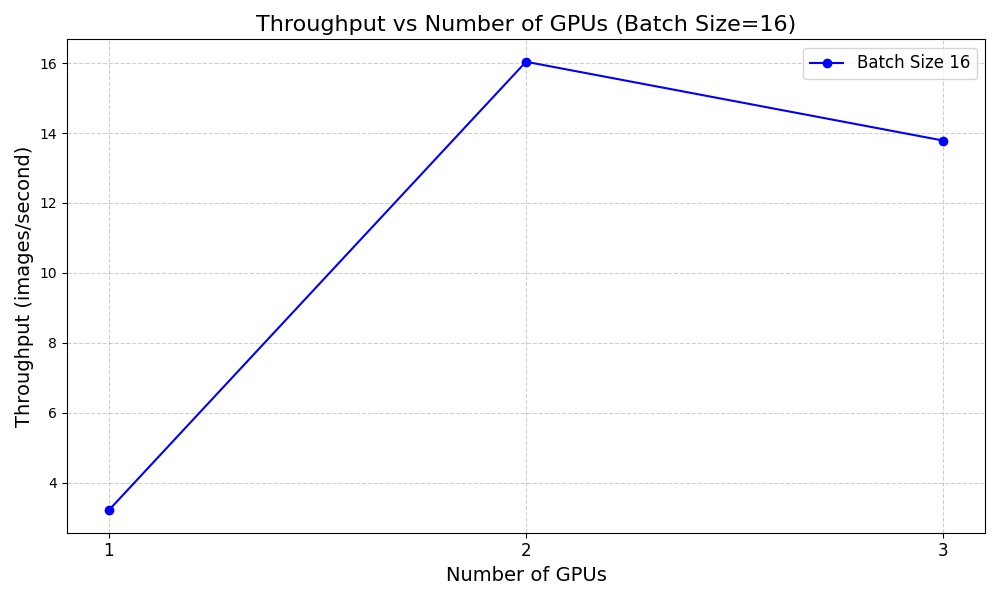
\includegraphics[width=0.8\textwidth]{GPU/throughput_bs16.png}
        \caption{Throughput vs number of GPU devices for a batch size of 16.}
        \label{fig:throughput_bs16}
    \end{figure}
\newpage
    \item \textbf{Batch Size = 64}:
    \begin{figure}[h!]
        \centering
        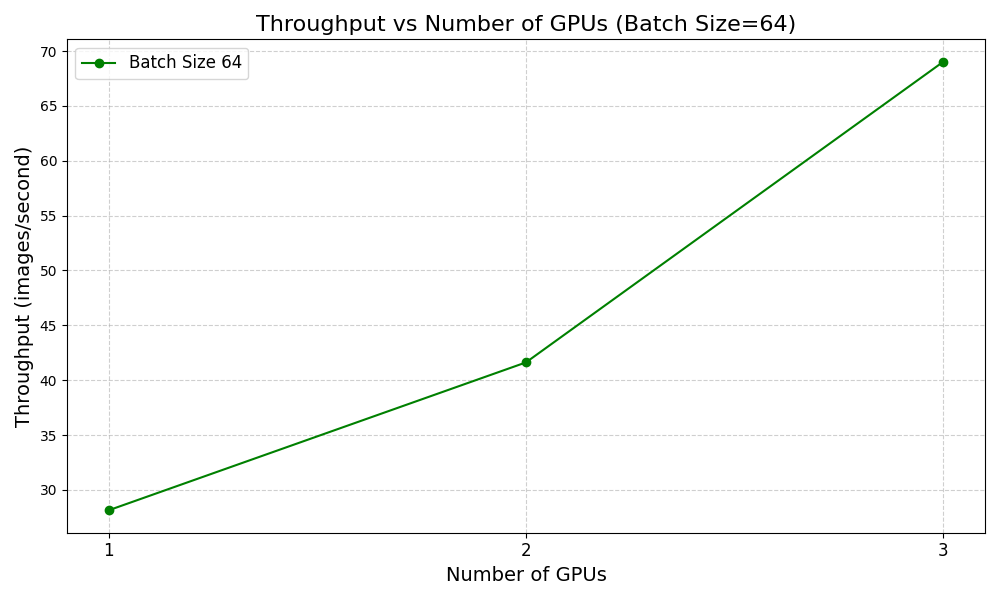
\includegraphics[width=0.8\textwidth]{GPU/throughput_bs64.png}
        \caption{Throughput vs number of GPU devices for a batch size of 64.}
        \label{fig:throughput_bs64}
    \end{figure}

    \item \textbf{Batch Size = 128}:\\
    \begin{figure}[h!]
        \centering
        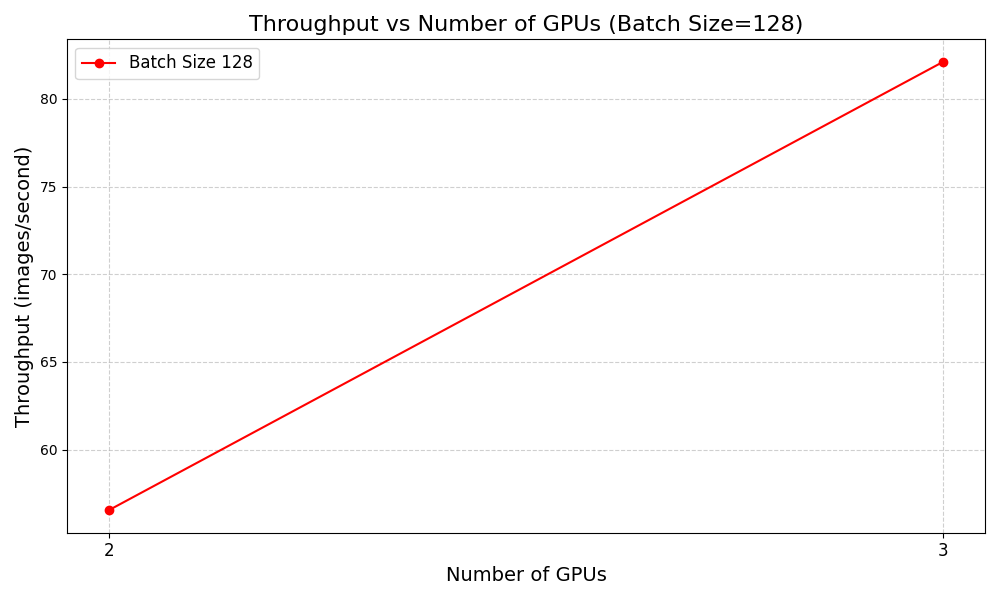
\includegraphics[width=0.8\textwidth]{GPU/throughput_bs128.png}
        \caption{Throughput vs number of GPU devices for a batch size of 128.}
        \label{fig:throughput_bs128}
    \end{figure}
\end{itemize}
\newpage
\subsection{Optimal number of GPUs vs batch sizes}
The following plot shows the optimal number of GPUs for different batch sizes, based on the throughput results.

\begin{figure}[h!]
    \centering
    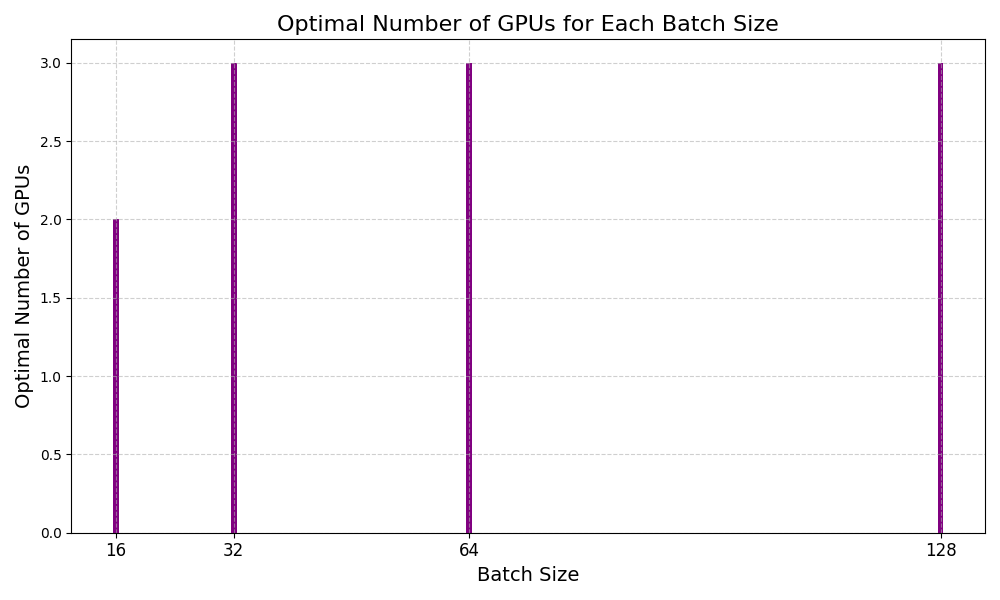
\includegraphics[width=0.8\textwidth]{GPU/optimal_gpus.png}
    \caption{Optimal number of GPUs for different batch sizes.}
    \label{fig:optimal_gpus}
\end{figure}

\subsection{Analyses}
\subsubsection{Throughput analysis}
\begin{itemize}
    \item \textbf{Batch Size = 16}: as shown in Figure \ref{fig:throughput_bs16} for a batch size of 16, the throughput increases significantly when moving from 1 to 2 GPUs, but it decreases slightly when using 3 GPUs. This behavior can be attributed to the communication overhead between GPUs, which becomes more pronounced with smaller batch sizes. While 2 GPUs provide a substantial improvement in throughput, adding a third GPU introduces additional overhead that outweighs the benefits for this batch size.
    
    \item \textbf{Batch Size = 64}: Figure \ref{fig:throughput_bs64} shows that for a batch size of 64, the throughput scales effectively with the number of GPUs. Moving from 1 to 2 GPUs results in a significant increase in throughput, and adding a third GPU further improves performance. Larger batch sizes like 64 allow for more efficient utilization of GPU resources, reducing the relative impact of communication overhead and enabling better scaling.

\item \textbf{Batch Size = 128}: as Figure \ref{fig:throughput_bs128} shows, the throughput for a batch size of 128 with only one GPU is missing because the experiment could not be completed on a single GPU due to \textbf{insufficient memory}\footnote{See the error output details.}. The DenseNet121 model, combined with a large batch size, exceeds the available GPU memory (10.91 GiB). However, distributed training across multiple GPUs resolves this issue by splitting the batch:
\begin{itemize}
    \item With 2 GPUs: The batch is split into 64 images per GPU, resulting in a throughput of nearly 55 images per second.
    \item With 3 GPUs: The batch is split into approximately 43 images per GPU, resulting in a throughput of nearly 85 images per second.
\end{itemize}
This demonstrates that distributed training is essential for handling large batch sizes, as it not only resolves memory limitations but also improves throughput significantly.


\textbf{Error Output:}
\begin{lstlisting}[basicstyle=\small\ttfamily, breaklines=true]
[rank0]: torch.OutOfMemoryError: CUDA out of memory. Tried to allocate 184.00 MiB. GPU 0 has a total capacity of 10.91 GiB of which 39.19 MiB is free. Including non-PyTorch memory, this process has 10.85 GiB memory in use. Of the allocated memory 10.55 GiB is allocated by PyTorch, and 41.14 MiB is reserved by PyTorch but unallocated.
\end{lstlisting}
\end{itemize}

\subsubsection{Optimal Number of GPUs Analysis}
\begin{itemize}
    \item Figure \ref{fig:optimal_gpus} shows the optimal number of GPUs for different batch sizes. For smaller batch sizes (e.g., 16), the optimal number of GPUs is 2. This is likely because the communication overhead outweighs the benefits of adding a third GPU for such a small batch size. 
    \item For larger batch sizes (e.g., 32, 64, and 128), the optimal number of GPUs is 3. This is because larger batch sizes allow for more efficient utilization of GPU resources, reducing the relative impact of communication overhead. As a result, adding more GPUs significantly improves throughput, making 3 GPUs the optimal configuration for these batch sizes.
\end{itemize}

\section{Code for the plots and registered time file}
The code used to generate the plots and the registered time file (CSV) are available in the following GitHub repository: \url{https://github.com/yisola2/Parallel}.

\section{Conclusion}
The results of the experiments demonstrate the benefits of parallelizing the training process for machine learning models. The use of multiple computing devices significantly reduces the training time, especially for larger batch sizes. The optimal number of devices varies depending on the batch size, and the results provide insights into the trade-offs between computational resources and training efficiency.

\section*{References}
\begin{itemize}
    \item NEF Cluster Documentation: \url{https://wiki.inria.fr/ClustersSophia/Clusters_Home}
    \item PyTorch Models: \url{https://pytorch.org/vision/0.9/models.html}
    \item Understanding DenseNet121: \url{https://medium.com/deepkapha-notes/implementing-densenet-121-in-pytorch-a-step-by-step-guide-c0c2625c2a60}
    \item Node Details: \url{https://wiki.inria.fr/ClustersSophia/Hardware}
    \item Cluster Usage Guide: \url{https://wiki.inria.fr/ClustersSophia/FAQ_new_config}
\end{itemize}

\end{document}